\documentclass[french]{report}
\usepackage[utf8]{inputenc}
\usepackage[T1]{fontenc}
\usepackage{babel}
\usepackage{fancyhdr}
\usepackage{graphicx}
\usepackage{color}
\usepackage{float}
\usepackage{hyphenat}
\hyphenation{mathéma-tiques récu-pérer}
\usepackage{imakeidx}
\makeindex[ intoc]
\usepackage[a4paper,left=1cm,right=1cm,top=1.8cm,bottom=1.8cm]{geometry}
\renewcommand{\chaptermark}[1]{\markboth{#1}{}}
\fancyhf{}
\fancyhead[LE,RO]{\leftmark}
\fancyhead[RE,LO]{\chaptername \thechapter}
\fancyfoot[CE,CO]{\chaptername \thechapter \leftmark}
\fancyfoot[LE,RO]{\thepage}
\setlength{\parindent}{4em}
\setlength{\parskip}{1em}
\renewcommand{\baselinestretch}{1.5}

\begin{document}
\tableofcontents

\baselineskip=2.0pt
\renewcommand*{\thepage}{\arabic{page}}%
\setcounter{page}{1}%
\newpage
\begin{center}
\section*{\huge Introduction Général}
\end{center}
\par
\LARGE Le succès de la messagerie électronique sous toutes ses formes n'est plus à démontrer. \\
Ce succès a participé, ces dernières années,au formidable développement du réseau Internet et il est difficile, aujourd'hui, de se passer de cet outil.\\ 
Les possibilités offertes par ce service sont la raison principale de ce succès.\\ 
Nous pouvons échanger de l'information avec quiconque possède un système standard.\\
Ces échanges, sous forme de messages électroniques simples ou bien complexes (avec des pièces jointes), sont réalisés avec une grande rapidité d'acheminement et sans la contrainte géographique des destinataires.\\
La capacité d'envoi d'un message à des destinataires multiples est également un atout important par rapport aux limitations du courrier postal,imposant pour sa part un message par destinataire.\\
Toutes ces fonctionnalités ont contribué à une large adoption de la messagerie par les particuliers. 
Cette dépendance est encore plus marquée dans l'environnement professionnel.\\
La messagerie électronique a pris la place des autres systèmes comme le fax ou le courrier postal.
Ce succès masque toutefois d'importantes lacunes.\\
La messagerie électronique a été adoptée sans réelle conscience des risques, des inconvénients et souvent dans la méconnaissance des lois.\\
\begin{titlepage}
\begin{titlepage}
\renewcommand*{\thepage}{\arabic{page}}%
\setcounter{page}{4}%
\chapter{
\textit{ État De L'art }
 }
\end{titlepage}
\renewcommand{\chaptermark}[1]{\markboth{#1}{}}
\pagestyle{fancy}
\renewcommand*{\thepage}{\arabic{page}}%
\setcounter{page}{5}%
\section{\LARGE Introduction}     
\LARGE Dans ce chapitre, nous décrivons le contexte général du projet. \\Nous présentons d’abord la définition de messagerie électronique,son histoire,importance et ses caractéristiques. 
\subsection{\LARGE Présentation De Messagerie Électronique :}
\LARGE Un courrier électronique, un courriel, un mail ou un e-mail est un message écrit envoyé électroniquement via un réseau informatique.\\ 
On appelle messagerie électronique l'ensemble du système qui permet la transmission des courriers électroniques. Elle respecte des règles normalisées afin d'autoriser le dépôt de courriels dans la boîte aux lettres électronique d’un destinataire choisi par l'émetteur.\\ \\
Pour émettre ou recevoir des messages par courrier électronique, il faut disposer d’une adresse électronique et d'un client de messagerie (ou d’une messagerie web permettant l'accès aux messages via un navigateur web).\\ L’acheminement des courriels, qui peuvent contenir des documents, est régi par diverses normes concernant aussi bien le routage que le contenu. Toutefois, comme le destinataire ne reçoit pas une copie conforme de l’écran de l’expéditeur, il est d'usage de respecter certaines règles implicites lors de l’envoi. De même, la connaissance de certains aspects techniques permet d’éviter des erreurs de compréhension ou de communication.\\ \\ En France, malgré les difficultés liées à son caractère souvent non (explicite patronyme absent), l'adresse électronique tend à être reconnue comme moyen valide de contacter une personne. En matière de droit des obligations, selon le code civil français $\ll$ l'écrit sur support électronique a la même force probante que l'écrit sur support papier $\gg$ . L'écrit électronique est de plus reconnu par le code civil comme valide à titre de preuve afin de conclure un contrat.En matière de droit social, est reconnu pour le salarié le $\ll$ droit, même au temps et au lieu de travail, au respect de l'intimité de sa vie privée $\gg$, ce droit impliquant $\ll$ en particulier le secret des correspondances $\gg$.\\ \\ Par leur contenu et leur forme, les messages envoyés par courrier électronique donnent à leurs destinataires une image de l'expéditeur. Le rôle du courrier électronique est croissant dans le maintien des liens sociaux, surtout en cas d'éloignement géographique.
\subsection{\huge Histoire:}
\subsubsection{\LARGE Préhistoire}
\LARGE On considère souvent que l’histoire de l’email (ou courrier électronique) débute en 1965, à une époque ou Internet n’existait pas encore. C’est en effet durant cette année que furent mis en place les premiers échanges de messages entre utilisateurs sur des réseaux privés.\\ \\
L’un des premiers systèmes ayant autorisé l’échange de messages fut le Compatible Time-Sharing System (CTSS) de la fameuse Institut de Technologies du Massachusetts (MIT), bien que cette paternité lui soit aussi revendiquée par la société System Development Corporation (SDC) et son propre Time-Sharing System (Système de Temps Partagé) créé pour le Q32, un ordinateur spécialement fabriqué par IBM pour l’Armée de l’Air américaine.\\ \\
Cela étant, le courrier électronique ne naît véritablement qu’à partir de la création du réseau ARPAnet, l’ancêtre d’Internet. Et c’est à l’automne 1971 qu’un ingénieur du nom de Ray (Raymond Samuel) Tomlinson, travaillant chez Bolt Beranek and Newman Technologies (société employée par le Ministère américain de la Défense pour le développement du réseau ARPA), s’envoya à lui-même le premier email de l’Histoire.\\ \\
Auparavant, les messages ne pouvaient être envoyés qu’aux utilisateurs d’un même domaine et consultés, le plus souvent, sur la même machine que celle qui servait à écrire et déposer les messages.
\subsubsection{\LARGE Genèse d’une révolution}
\LARGE Ray Tomlinson conçu une application spécifique à l’envoi de messages, SNDMSG (Send Message), ainsi qu’une application dédiée à la lecture de ces derniers, READMAIL. Ces applications autorisaient la lecture de messages par différents utilisateurs mais sur une seule et même machine. L’idée de Ray Tomlinson fut d’ajouter à ces applications un protocole d’envoi et de réception de fichiers à travers le réseau ARPAnet, le CPYNET.\\ \\
Après l’écriture de quelques 200 lignes de code et la création de deux boîtes électroniques sur deux machines côte à côte, Ray Tomlinson devait encore trouver un moyen pour que le programme différencie facilement un message local d’un message réseau. C’est alors qu’il eut l’idée de dissocier nom d’utilisateur et nom d’hôte avec le seul caractère qui n’était utilisé dans aucun nom propre ni, et surtout, dans aucun nom d’entreprise – qui, par la suite, pouvait servir de préfixe au nom de domaine : le symbole @ (arobase).\\ \\
Ray Tomlinson parvient ainsi à s’envoyer le premier $\ll$ netmail $\gg$ de test avec pour seul contenu $\ll$ QWERTYUIOP $\gg$, soit la première ligne de caractère du clavier anglophone.\\ \\
Le premier véritable email envoyé à des utilisateurs le fut par Ray Tomlinson pour annoncer justement la naissance de son application et en expliquer son fonctionnement aux employés de BBN Technologies.
\subsubsection{\LARGE A star is born}
\LARGE L’email connu un tel succès qu’il devint vite inenvisageable, pour les utilisateurs du réseau ARPAnet, de s’en passer. En conséquence, le logiciel obtint très vite le qualificatif de $\ll$ killer app $\gg$ (ou $\ll$ application-qui-tue $\gg$) du réseau ARPAnet, et les développeurs s’attachèrent soit à améliorer le programme et son protocole de transfert, soit à développer leurs propres solutions.\\ \\
Dès 1973, une étude menée par l’ARPA dévoilait que 75\% du trafic de son réseau était généré par l’échange d’emails.\\ \\
C’est en 1975 que l’email va se voir adjoindre un véritable client de messagerie avec la création de MSG par John Vittal, alors ingénieur à l’Institut des Sciences de l’Information, dans l’Université de Californie du Sud. Son programme, considéré comme l’ancêtre des clients de messagerie modernes comme Outlook ou Thunderbird, permet à lui seul de rassembler les fonctions de lecture, d’envoi, de transfert des mails, d’adjonction de pièces jointes et la notion de $\ll$ corbeille $\gg$ pour les messages supprimés, le tout dans une interface simplifiée.\\ \\
Dans la même année, la liste de diffusion non-officielle $\ll$ SF-Lovers $\gg$, pour les amoureux de la science-fiction, devient la plus populaire de tout le réseau ARPA.
\subsubsection{\LARGE Le côté obscur du mail}
\LARGE En 1978, Gray Thuerk, un employé de Digital Equipment Corporation (sous-traitant pour le Ministère américain de la Défense), souhaite faire connaître l’un des nouveaux produits de sa société aux ingénieurs du réseau ARPAnet. C’est dans le but de ce simplifier la tâche d’envoi du même mail pour chaque personne que Gray Thuerk récupérera les adresses mail de toutes les 393 personnes, connectées à l’époque sur le réseau, pour leur transmettre ce qui est aujourd’hui considéré comme le premier spam de l’histoire. Son action fut critiquée par l’ARPA, jugeant l’annonce commerciale inappropriée avec l’utilisation qui devait être faite du réseau, à l’origine prévue pour la recherche et le développement technologique.
\subsection{\LARGE L’importance de l‘ e-mail}
\LARGE E-mail, ou par courrier électronique comme il est communément connu est un moyen de communication très populaire dans le monde entier. Auparavant, les gens utilisaient pour communiquer avec eachother en utilisant des lettres et des cartes postales, mais ce Lorsque email abord présenté, il a complètement révolutionné la façon dont Appelez les gens utilisés pour communiquer avec eachother. Alors que les gens ont dû attendre pendant des jours avant Leurs lettres ont été reçues et ont répondu à succès, email fait une question de minutes. Maintenant, le courriel est devenu une recherche de partie cruciale de notre vie a fait que nous ne pouvons pas vraiment vivre sans elle. Voici quelques conseils ont fait souligner l’importance de l’email:
\subsubsection{\LARGE Email est très rapide}
\LARGE Communication par courriel est très rapide, beaucoup plus rapide que les lettres standard, etc. Des informations détaillées peuvent être envoyés, lu et répondu à un email, avec aussi peu de tracas que possible. Aujourd’hui, quand le temps est de l’essence, email connectivité joue un rôle majeur car elle permet aux utilisateurs d’envoyer des messages et d’obtenir des réponses en aussi peu de temps que possible.
\subsubsection{\LARGE Email est libre}
\LARGE Alors que l’envoi de lettres et de cartes postales des frais requis, l’envoi de courriels ne sont pas à la charge du tout; Il est totalement gratuit. Doté d’une connexion serveur de messagerie: tel que Gmail, AOL, Yahoo, Outlook et d’autres clients de messagerie gratuits, la création simple récit à l’e-mail est extrêmement. Plus important encore, l’envoi ou la réception de courriels est entièrement gratuit. Même les services comme Zimbra email ne vous permettent de fixer votre propre nom de domaine à vos messages et inclure des services de cloud computing peut être consulté gratuitement.
\subsubsection{\LARGE Email peut être envoyé à de nombreuses personnes à la fois:}
\LARGE Le courrier électronique est l’un des modes les plus importants de la communication sont utilisés à des fins de marketing a fait. Selon les résultats de l’enquête de marketing de l’année dernière, environ soixante pour cent de la commercialisation sur l’Internet a été fait par courriel. Email marketing a prouvé être très efficace, même en raison de l’introduction de filtres anti-spam et de divers autres types de filtre anti-spoofing, le marketing par courriel est avérée silencieuse Un des types les plus efficaces de marketing sur Internet.
\subsubsection{\LARGE Email Fournit une communication efficace pour les entreprises et les employés}
\LARGE Maintenant, les employés doivent être mis au courant de l’évolution de la société sur base immédiate. Merci à l’email, cela peut se faire assez facilement. Les entreprises peuvent envoyer des e-mails à leurs employés sur la route, permettant une communication efficace entre les employés et l’administration.
\subsubsection{\LARGE Fournit Email efficace Mobile Communication}
\LARGE Android, iOS et Blackberry tous offrent des options de connectivité sans faille et vous permettent de synchroniser vos comptes de messagerie. Cela rend beaucoup plus facile pour les gens à envoyer et recevoir des e-mails sur leurs téléphones mobiles seulement, permettant une communication efficace. M. électronique vous permet de synchroniser votre e-mail Zimbra avec le mobile ainsi, grâce à notre partenariat avec ZeXtra.\\ \\
L’importance de l’e-mail ne peut pas être sous-estimée suffisante, principalement parce qu’il est devenu important de rechercher le mode de communication dans tous les domaines et industries. Parce que toutes les conversations de messagerie sont enregistrées, de sorte qu’il offre enregistrement des conversations, le rendant parfait pour un usage professionnel.
\section{\LARGE Les Principaux concepts: }
\subsection{\LARGE Protocoles de communication (de transport)}
\LARGE Le fonctionnement du courrier électronique repose aussi sur une série de protocoles de communication destinés à envoyer ses messages, de serveur à serveur, à travers l'Internet. Les principaux protocoles sont les suivants : SMTP, POP3 ou encore IMAP4, chacun jouant un rôle bien précis.\\ \\

\subsubsection{\LARGE Le protocole SMTP }
\LARGE Le protocole SMTP (Simple Mail Transfer Protocol) est le protocole standard permettant de transférer le courrier entre deux serveurs de messagerie - celui de l'expéditeur et celui du destinataire.\\ \\
Le protocole SMTP spécifie aussi l'entête des courriers (from :, to :, etc...), les possibilités d'envoi groupé, la gestion des heures ou encore le format des adresses des utilisateurs. Ainsi, avant chaque envoi de message, SMTP vérifie auprès des différents FAI (Fournisseurs d'accès à Internet) que l'adresse du destinataire existe réellement. Si tel n'est pas le cas, le message revient automatiquement dans la boîte aux lettres de l'expéditeur.
Un message met en général quelques secondes seulement pour aller d'un point à un autre sur l'Internet. Le message peut transiter par différents relais ou par un seul serveur si le destinataire utilise le même serveur de messagerie que l'expéditeur.\\ \\
Dans un logiciel de courrier, il faut toujours donner l'adresse de son serveur SMTP qui prendra généralement la forme suivante : smtp.nom$\_$de$\_$domaine ou mail.nom$\_$de$\_$domaine\\ \\
Exemple : smtp.google.com.

\subsubsection{\LARGE Le protocole POP }
\LARGE Le protocole POP (Post Office Protocol) permet d'aller récupérer son courrier sur un serveur distant (le serveur POP). Ce protocole est nécessaire pour les personnes qui ne sont pas connectées en permanence à l'Internet. Ainsi, POP3 permet le traitement hors-ligne de ses emails. Il suffit de se connecter périodiquement à son serveur de messagerie, via un logiciel spécifique, pour rapatrier sur sa machine le courrier en attente. Les messages récupérés sont ensuite effacés du serveur de messagerie, sauf configuration contraire du logiciel de messagerie. Il est, en effet, possible de laisser une copie des messages sur le serveur.\\ \\
POP gère aussi l'authentification à l'aide d'un nom d'utilisateur et d'un mot de passe. Par ailleurs, ce protocole bloque la boîte aux lettres, à chaque connexion au serveur de messagerie. Ceci afin de rendre impossible une consultation simultanée par deux utilisateurs d'un même compte e-mail.
Mais ce protocole n'est, en revanche, pas sécurisé car les mots de passe - comme les e-mails - circulent $\ll$ en clair $\gg$ (le contenu n'est pas crypté) sur le réseau. A titre de comparaison, c'est comme si nous prenions l'habitude d'envoyer nos lettres sans prendre la peine de les insérer dans une enveloppe.\\ \\
Dans un logiciel de courrier, il faut toujours donner l'adresse de son serveur POP qui prendra généralement la forme suivante : pop.nom$\_$de$\_$domaine.

\subparagraph{\LARGE Ainsi, l'utilisateur du courrier électronique met en oeuvre, en général, conjointement deux protocoles : SMTP et POP3. Il envoie des messages en utilisant SMTP (protocole d'envoi) et il récupère les nouveaux messages en utilisant POP3 (protocole facteur). Enfin, entre chaque serveur - celui de l'expéditeur et celui du destinataire - fonctionne encore le protocole SMTP qui a la charge de réceptionner les mails sur le serveur de messagerie. C'est la raison pour laquelle on parle de serveur de messagerie SMTP.}
\subparagraph{
\LARGE L'évolution du courrier électronique vers le multimédia et le manque de flexibilité de POP favorisent l'émergence d'un nouveau protocole : l'IMAP.}

\subsubsection{\LARGE Le protocole IMAP (Interactive Mail Access Protocol)}
\LARGE Le protocole IMAP (Interactive Mail Access Protocol), moins utilisé que POP, offre plus de possibilités. Cependant, de plus en plus de FAI utilisent ce protocole. IMAP4 pourrait, à terme, remplacerh  progressivement POP3.\\ \\
La principale innovation de IMAP4 réside dans la possibilité de gérer son courrier directement sur le serveur de son FAI. Tous les courriers et dossiers de messages restent sur le serveur. A chaque connexion au serveur par IMAP4, l'utilisateur n'effectue donc plus une relève des messages mais plutôt une synchronisation des messages. Le logiciel affiche alors une copie de sa boîte aux lettres, archives comprises.\\ \\
En outre, il n'est plus nécessaire de rapatrier ses messages sur son ordinateur. Ainsi, l'on peut désormais télécharger uniquement les messages de son choix. Les autres peuvent être supprimés quand ils ne restent pas tout simplement stockés sur le serveur du FAI.\\ \\
Par ailleurs, un autre avantage tient dans la possibilité de consulter sa messagerie depuis des ordinateurs différents et de retrouver la même organisation puisque les messages restent stockés sur le même serveur. IMAP4 est ainsi utile à toutes les personnes qui se déplacent et désirent pouvoir consulter facilement leur compte e-mail.\\ \\
IMAP4 permet donc de gérer plusieurs accès simultanés, d'administrer plusieurs boîtes aux lettres et de trier le courrier selon plus de critères. Il est ainsi possible de manipuler des dossiers présents sur le serveur comme s'ils étaient sur le poste-client, permettant l'organisation personnelle d'une boîte-aux-lettres.


\subsubsection{\LARGE Protocoles de contenu}
\LARGE
Historiquement, la messagerie Internet a été conçue pour transférer du texte en ASCII US (American Standard Code for Information Interchange) simple, c'est-à-dire sur 7 bits. C'est la raison pour laquelle il a fallu trouver des solutions pour transférer des informations binaires (images, sons, etc...) et des messages écrits dans une langue nécessitant plus de 7 bits pour coder son alphabet. Par exemple, l'envoi de textes contenant des accents nécessite un codage sur 8 bits et donc une extension du format ASCII d'origine.\\ \\
Pour réaliser cette intégration des jeux de caractères 8 bits, divers systèmes d'encodage ont alors vu le jour : BinHex (essentiellement sur Mac), UUencode (essentiellement sur Unix) et surtout MIME (Multi-purpose Internet Mail Extensions) qui s'est imposé comme standard et qui est exploité par la plupart des logiciels de messagerie.\\ \\
MIME est une spécification d'Internet, permettant d'échanger des textes écrits dans des langues différentes (et utilisant des ensembles de caractères différents) ainsi que des documents de tous types (images, sons, vidéos...), entre des machines de systèmes différents (PC, Mac, Linux, Unix, etc...).\\ \\
Avec MIME, il est donc désormais possible d'envoyer des messages contenant des caractères accentués, du texte enrichi (gras, souligné, en couleurs, etc...), des images, du son, de la vidéo, des programmes, des $\ll$ pointeurs $\gg$ de fichiers (URL), etc...  .\\ \\
\subsection*{\LARGE Comment fonctionne MIME ?}
\LARGE Ce protocole utilise essentiellement deux encodages : Le Quoted-Printable (QP) et Le Base64. Le premier permet de coder tout alphabet nécessitant plus de 7 bits, le second étant plutôt utilisé pour les fichiers binaires envoyés en pièce jointe.\\ \\
MIME prend donc en charge chaque message électronique. Il en encode les différentes parties - corps du texte et/ou pièces jointes - et place dans l'entête les informations nécessaires afin que le logiciel qui réceptionne le message puisse le décoder et rétablir ainsi la lisibilité du fichier.\\ \\
Il suffit simplement que le logiciel de messagerie du destinataire soit aussi équipé de l'extension MIME.
\newpage
\section{\LARGE Étude Des Exemple:}
\subsection{\LARGE Messagerie Électronique Gmail}
\LARGE Gmail est un fournisseur de courrier électronique,Ce service est proposé par Google, et permet de gérer vos emails depuis votre navigateur Internet (webmail) ou depuis n’importe quelle application (PC, Mac, Mobile).
\subsubsection{\LARGE Histoire}
\LARGE
\textbf{Début 2007}. Google abandonne son système d’invitation pour Gmail. Tout internaute peut directement ouvrir un compte Gmail.\\ \\
\textbf{Octobre 2008}. Lancement de la première application Gmail sur Android.
\textbf{Juillet 2009}. Après plus de 5 ans de développement et d’améliorations, Google sort Gmail et toutes les Google Apps de leur $\ll$ phase d’expérimentation $\gg$. Gmail n’est plus en version bêta.
\textbf{Août 2009}. Avec 37 millions de visiteurs uniques (+25 \% sur un an) (source ComScore), Gmail devient numéro 3 aux USA, derrière Yahoo Mail et Hotmail.\\ \\
\textbf{Septembre 2010}. Lancement de la boîte de réception prioritaire (Priority Inbox en VO) : les messages que Gmail juge prioritaires pour vous peuvent être mis en avant dans la boîte de réception. (Lire Avec la boîte de réception prioritaire, Gmail identifie pour vous les e-mails importants).
\textbf{Novembre 2011}. Google généralise la nouvelle interface de Gmail. Par ce relooking, Google corrige les imperfections et les aspects un peu vieillots de l’interface du webmail. (Lire La nouvelle interface de Gmail passée au crible).\\ \\
\textbf{Mai 2012}. Gmail devient numéro un de la messagerie, avec 425 millions d’utilisateurs actifs, devant Hotmail (350 millions) et Yahoo! Mail (310 millions). (Source : PC INPact).
\subsubsection{\LARGE Fonctionnement}
\LARGE Le fonctionnement de Gmail est très simple puisqu’il se base sur les protocoles email standards (POP, IMAP et SMTP)
\newpage
\subsubsection{\LARGE Fonctionnalités}
\LARGE L’innovation de Google était principalement dans l’interface et ses fonctionnalités additionnelles :
\begin{itemize}
    \item[•	Tri des emails grâce à des filtres poussés]
    \item[•	Moteur de recherche avancé et efficace]
    \item[•	Regroupement des emails par conversation]
    \item[•	Répondeur automatique]
    \item[• Enregistrement de votre saisie au fur à mesure (aucune perte possible)]
    \item[•	Lien étroit et intégration avec les autres applications Google]
    \item[•	Antispam et antivirus intégré]
\end{itemize}
\subsection{\LARGE Messagrie Electronique Yahoo}
\LARGE Yahoo! Mail est une messagerie web gratuite, offerte par l'entreprise américaine Yahoo!. Il s'agit d'une application Web permettant de communiquer par courriers électroniques.
\subsubsection{\LARGE Histoire}
\LARGE \textsc{ Yahoo! Mail  a été créé en 1997  par Yahoo! La société américaine de service web après avoir étendu ses services.\\ \\
\textbf{Le 8 mars 1997}, Yahoo! a acquis la société de communication en ligne Four11. Le service de messagerie Web de Four11, Rocketmail, est devenu Yahoo! Mail.\\ \\
\textbf{2005}, Une nouvelle version comprenait une nouvelle interface Ajax, un glisser-déposer, une recherche améliorée, des raccourcis clavier, une saisie automatique d'adresse et des onglets. Cependant, d'autres fonctionnalités ont été supprimées, telles que les largeurs de colonne et un clic supprimer-déplacer-vers-suivant.\\ \\
\textbf{Mai 2007}, Yahoo ! annonce un stockage gratuit et illimité des e-mails.
En octobre 2010, Yahoo a publié une version bêta de Yahoo Mail qui comprenait des améliorations des performances, de la recherche et de l'intégration de Facebook.
\textbf{Mai 2011}, la version beta est devenu l'interface par défaut.
\textbf{Mai 2011} , Yahoo lance une nouvelle version avec une interface qui se rapproche de celle de Gmail et d’Outlook.com.\\ \\
\textbf{2013} , Yahoo! réduit le stockage «illimité» des e-mails .
\textbf{Octobre 2013}, Yahoo ! lance une nouvelle version qui a été vivement critiqué pour sa mise en page et sa capacité d'utilisation.}
\subsubsection{\LARGE Fonctionnement}
\LARGE Le fonctionnement de Yahoo ! Mail est très simple il se base sur \textbf{le protocole IMAP}.
\subsubsection{\LARGE Fonctionnalités}
\LARGE Yahoo! Mail vous permet de choisir parmi les 4 plans de messagerie différents, dont 3 plans personnels et 1 plan d'affaires. Les 3 plans personnels incluent les comptes Basic, Plus et Ad-Free. Basic Mail est la version la plus simple de Yahoo Mail où vous ne rencontrez pas de messagerie Yahoo complète. De plus, Mail est également connu sous le nom de messagerie complète, qui propose d'autres fonctionnalités telles que les pièces jointes par glisser-déposer, les GIF, les thèmes, les diaporamas de photos. En revanche, les comptes sans publicité ne montrent pas les publicités. Yahoo Mail Pro est un autre nom pour les comptes sans publicité.\\ \\
Vous pouvez utiliser un e-mail personnel pour vous connecter avec vos amis et votre famille et vos e-mails professionnels pour gérer votre entreprise et vos employés. L'e-mail professionnel est fourni avec votrenom@votre-entreprise.com. Alors que les e-mails personnels sont accompagnés de votrenom@domain.com. @yahoo.com,@ymail.com et @ rocketmail.com sont les trois domaines yahoo.\\ \\
Prend en charge les comptes de messagerie non Yahoo tels que Gmail, Outlook et AOL :
En 2015, Yahoo a annoncé qu'il prend en charge les comptes de messagerie non-yahoo. Ces comptes de messagerie non-yahoo incluent Gmail, Outlook et AOL. Yahoo propose ces 3 options dans le signe dans la page elle-même. Au lieu de vous connecter ou de vous inscrire, vous pouvez sélectionner l'un des 3 services Web pour accéder à Yahoo! Courrier.\\ \\
Yahoo! Mail prend en charge 37 langues différentes . L'arabe, le grec, le hongrois, le néerlandais et l'italien en sont quelques exemples. Différentes langues ont des codes différents.
Dès que vous créez un compte Yahoo! Compte de messagerie, vous disposez de 1 To de stockage en ligne gratuit. Ce stockage est plus que suffisant pour des millions de messages.\\ \\
Vous pouvez rédiger une réponse automatique à l'avance afin que lorsque les gens vous envoient des e-mails, ils soient informés que vous ne serez pas disponible pour répondre immédiatement au courrier.
\newpage
\section{\LARGE Étude comparative:}
\LARGE Il y avait des rapports de la mort de l'email est très vite quand la révolution Facebook a commencé sur Internet. Mais, l'évolution des sites de médias sociaux comme Facebook, Twitter et bien d'autres ont pas causé de brèche dans la popularité du service de courrier électronique. Même aujourd'hui, les gens utilisent le service de messagerie pour envoyer détails mails et des lettres à leurs amis, des parents ou des contacts d'affaires. Gmail est encore l'un des modes préférés de communication. Il vous donne la liberté de joindre des fichiers et dossiers importants ainsi que des liens internet avec votre courrier. Vous pouvez envoyer des messages ou recevoir des messages à partir de n'importe où dans le monde et à tout moment, à condition d'avoir une connexion Internet sur votre ordinateur. En utilisant un service de courriel, vous ne devrez pas la restriction de limiter vos messages à seulement 140 personnages comme ce que propose Facebook et Twitter. Donc, quel que soit dit, le courriel est là pour rester et nous allons discuter sur les deux services de messagerie électronique populaires sur le Web, Gmail et Yahoo Mail et comment ils se situent uns contre les autres.
\subsubsection{\LARGE T'chat options}
\LARGE Gmail vous donne la possibilité de chatter avec vos contacts à partir de votre boîte de réception, alors que cette fonctionnalité est proposée par Yahoo Mail. Yahoo Messenger doit être utilisé pour discuter avec vos amis et contacts. Aussi, Gmail propose un système de chat vocal et vidéo et aussi une envoyer des SMS à votre contact par courrier, qui est tout à fait novatrice et intéressante. Il n'y a pas de telles fonctionnalités sur l'offre de Yahoo Mail et il est purement un message d'envoi et recevoir des messages d'un service de messagerie électronique. Aussi, vous pouvez ouvrir plusieurs fenêtres de discussion sur Gmail à un moment et discuter à deux ou trois contacts à la fois.
\newpage
\subsubsection{\LARGE Sécurité}
\begin{itemize}
\LARGE
\item Gmail vous offre le meilleur sécurité et la confidentialité quand il vient à service e-mail.
\item Vous pouvez faire usage de la procédure de vérification en 2 étapes pour vous connecter à votre compte Gmail afin que personne ne sera en mesure d'accéder à votre compte Gmail facilement.
\item Vous serez invité à entrer un second mot de passe après que vous avez entré votre nom d'utilisateur et mot de passe pour vous connecter à votre compte Gmail.
\item Ce 2ND mot de passe sera envoyé un texto pour vous sur votre numéro de téléphone mobile enregistré.
\end{itemize}
\LARGE Il n'y a pas cette fonctionnalité sur l'offre dans Yahoo Mail. Aussi, Gmail a une plus petite séance heure d'expiration de Yahoo Mail et donc il offre une meilleure sécurité. Avec option d'affichage d'origine dans Gmail, vous pouvez vérifier l'adresse email réelle de l'expéditeur et vous empêcher les attaques de courrier phishing.
\subsubsection{\LARGE Publicité gratuite}
\LARGE Il ya quelques publicités qui apparaîtront sur Gmail comme one-liners-dessus de la boîte de réception en fonction des mails. Mais, si vous optez pour Yahoo Mail, puis vous verrez d'énormes annonces à venir dans les côtés de la boîte email Yahoo. En fait, vous pourrez également voir des publicités sur la page de connexion. Il n'y a pas de distraction tout en utilisant Gmail et vous ne serez jamais gêné par la publicité.
\subsubsection{\LARGE Tabbing automatique des messages}
\LARGE Il ya quelques onglets personnalisés que vous pouvez créer ou faire usage de Gmail comme sociaux, les promotions, primaire, mises à jour et ainsi de suite. Gmail jugera automatiquement quelle catégorie un courrier entrant tombe dans et enverra les mails dans la catégorie appropriée de sorte que vous ne le faites pas, ah recherche de veto pour un type particulier de courrier dans votre boîte de réception. Juste cliquez sur la catégorie de mise à jour pour obtenir les mises à jour de paiement, les messages Facebook, paiements de factures mobiles et ainsi de suite. Donc, avec cette fonctionnalité messages de spam ne seront pas recevables et seront automatiquement envoyé dans le dossier de spam. Le filtrage de spam offert par Gmail est plus puissant que ce que propose Yahoo Mail.
\subsubsection{\LARGE Conclusion}
\LARGE Il n'y a pas de doute que Gmail offre le meilleur service de messagerie par rapport à Yahoo Mail.\\
Dans le chapitre suivant, nous passerons à une étude de conception qui nous permettra de mieux concevoir l'architecture générale de notre projet ainsi que d'en identifier ses nécessités.
\end{titlepage}
\begin{titlepage}
\pagestyle{fancy}
\chapter{
\textit{ Étude conceptuelle }
}
\renewcommand*{\thepage}{\arabic{page}}%
\setcounter{page}{30}%
\newpage
\section{\huge Introduction}     
\LARGE Dans ce chapitre, nous présentons les différentes fonctionnalités que nous voulons voir figurer dans notre projet et détaillons si nécessaire, ainsi que la conception et modélisation de notre application avec ses différents parties.\\
\section{\huge La Conception de notre application :}
\LARGE Développer un système qui transmet et reçoit les données d'un utilisateur en temps réel soulève de nombreux problèmes et difficultés, dans cette étape nous avons voulu essayer d'éliminer ces problèmes et surmonter les difficultés pour nous assurer que notre application aura de bonnes performances.
Pour ce faire, nous avons dû identifier les principales parties interactives de notre projet qui sont: \\
\subsection{\LARGE Utilisateur}
\LARGE Après la première étape de création d'un compte utilisateur dans l'application, l'utilisateur aura un compte dans la base de données qui lui donnera la possibilité d'interagir avec les différentes parties de notre application.
Ce schéma représente les étapes nécessaires pour accéder et interagir avec les fonctionnalités de notre application : \\
\begin{figure}[H]
    \centering
    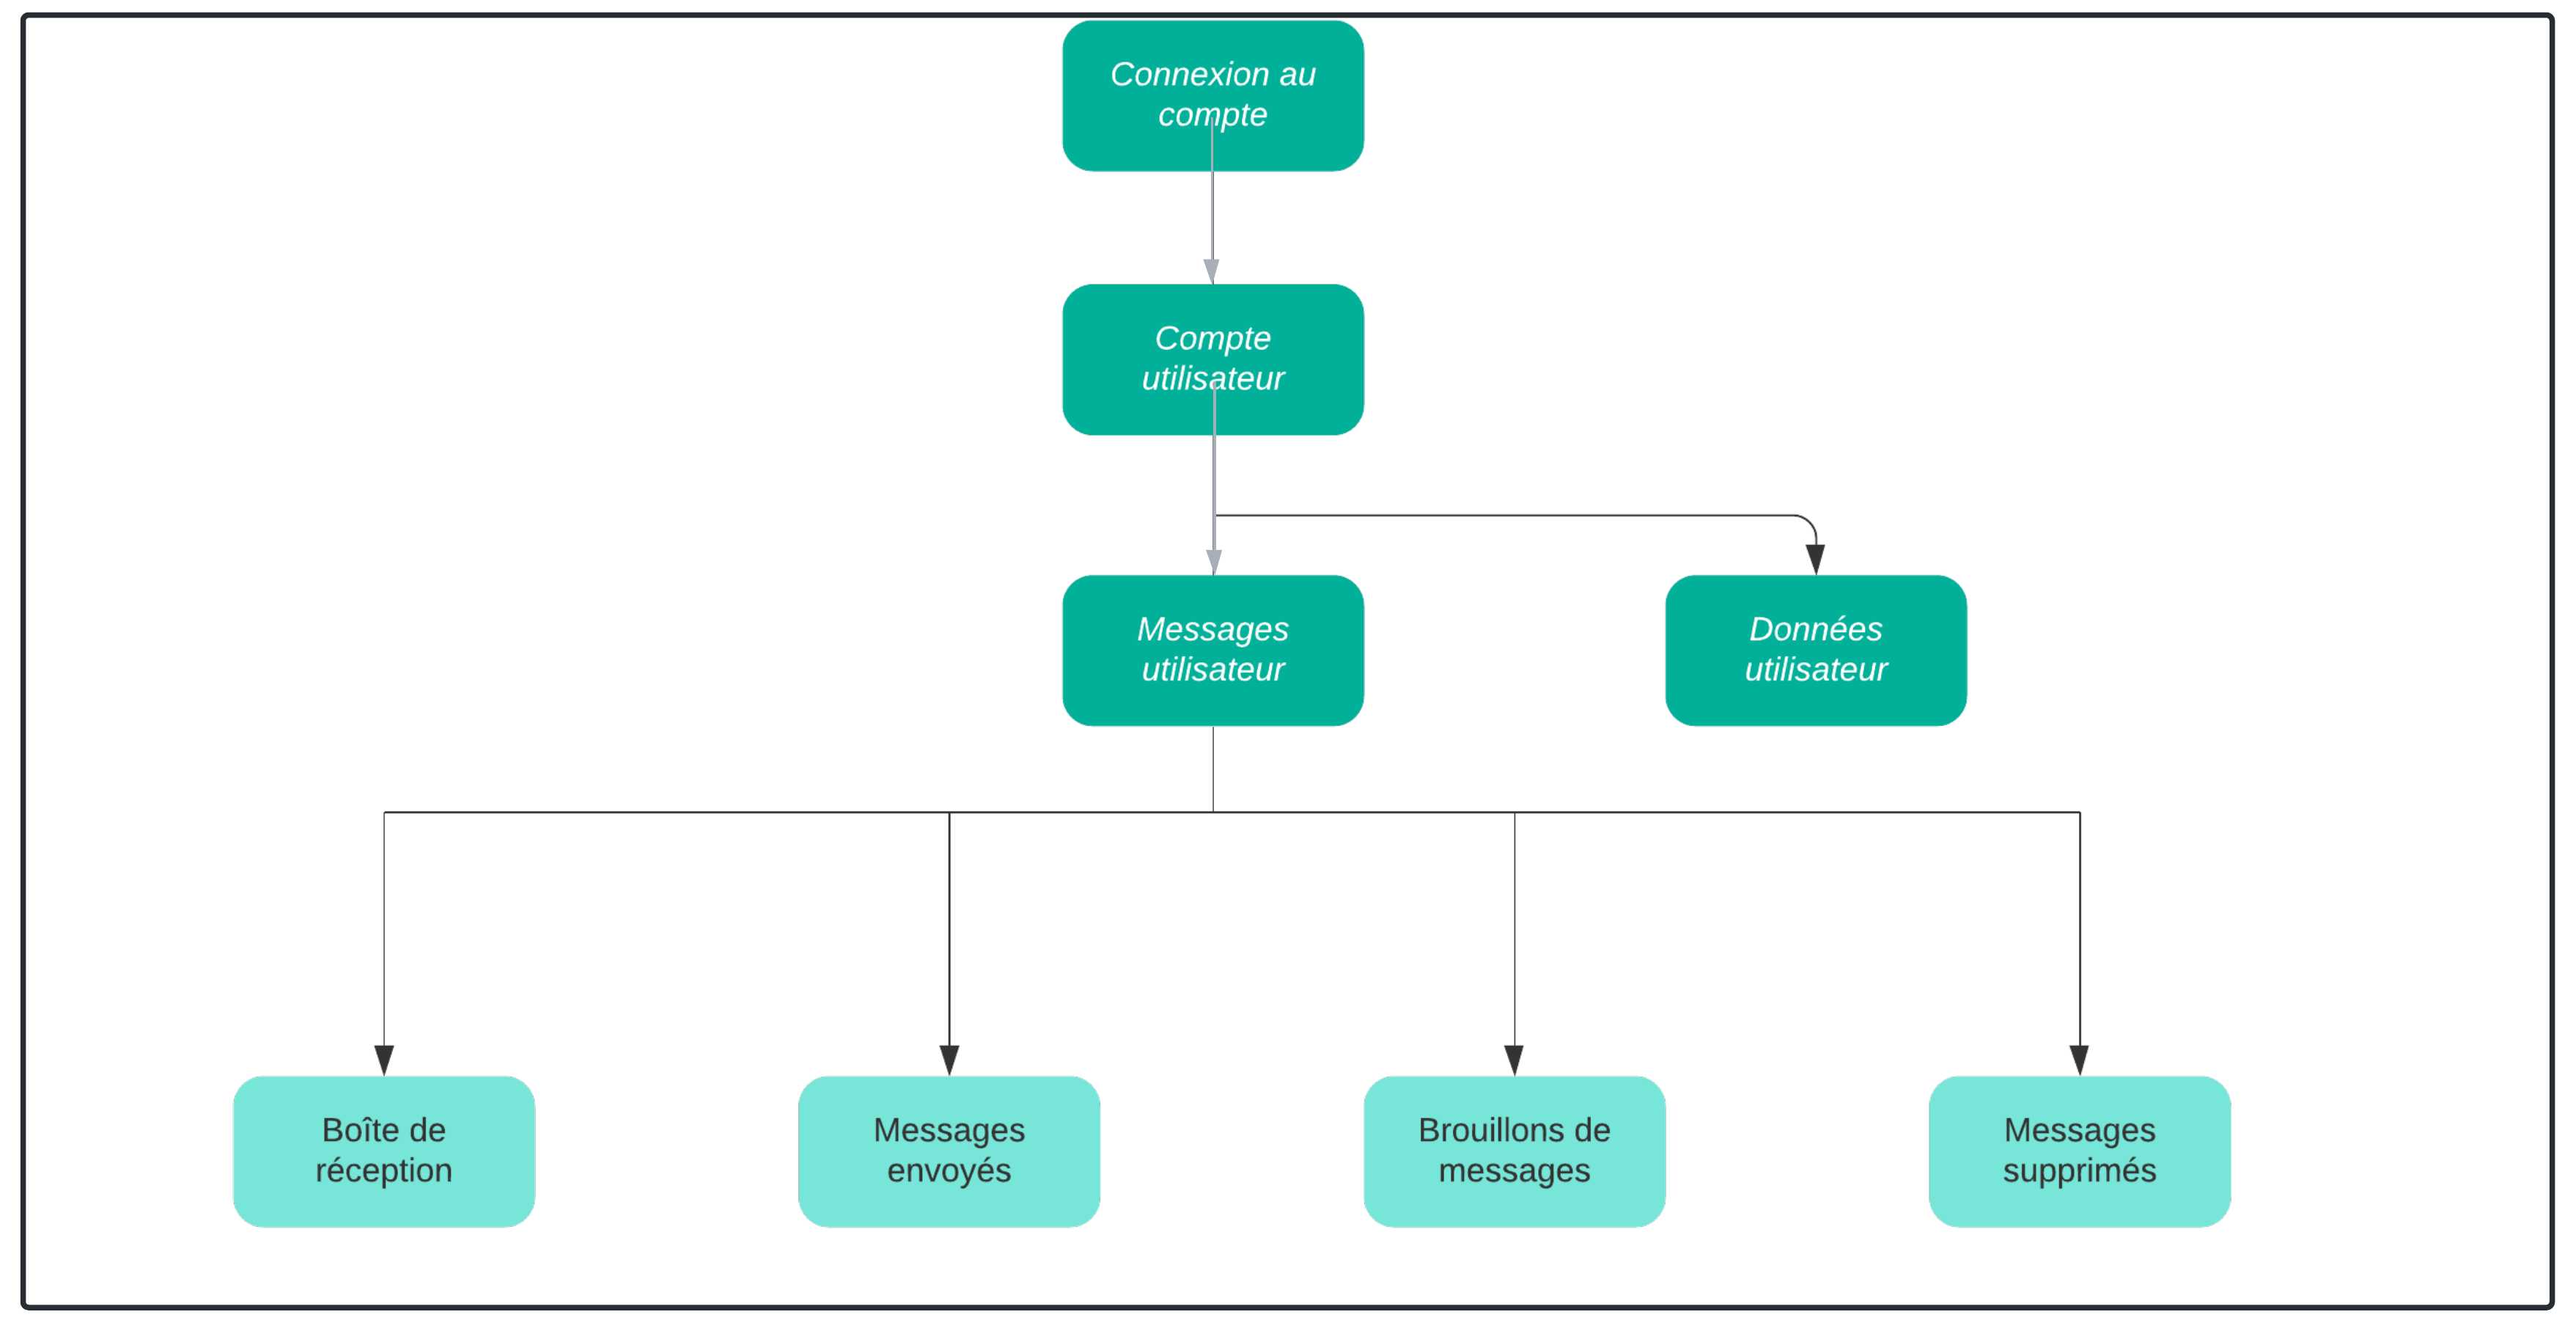
\includegraphics[width=0.88\textwidth]{Architecture de notre application}
    \caption{Architecture simplifiée de notre application}
    \label{fig:Architecture}
\end{figure}
\subsection{\LARGE Messages}
\LARGE Une collection de messages spécifiques à un utilisateur ou à plusieurs utilisateurs classés dans leur propre catégorie (reçus, envoyés, supprimés, brouillon).\\
Pour une application de messagerie, ce sont les données les plus cruciales, à cause de cela, nous avons dû choisir la meilleure construction de cette classe.\\
Dans notre application, un message ou un e-mail est une classe constitué de différents attributs notamment un identifiant message, contenu de message, destinataire, expéditeur ...\\
Voir la figure 2.2 pour la liste complète des attributs.\\
\subsection{\LARGE Base de données}
\LARGE La partie la plus importante de notre projet, l'accès en lecture ou en écriture aux données détermine la vitesse de performance de notre application, il peut donc limiter la fonctionnalité de notre application.\\
Pour cela, nous nous sommes assurés de choisir la meilleure structure pour notre base de données en mettant l'accent sur la vitesse et les performances optimales.\\
La figure ci-dessous montre une structure simplifiée de notre base de données.
Cette figure montre également la structure des parties principales de notre projet, les classes utilisateur et message ainsi que diverses autres classes nécessaires au fonctionnement de notre application.\\
Notre base de données est une base de données NoSQL, elle ne contient pas de tables.
\begin{figure}[H]
	\centering
    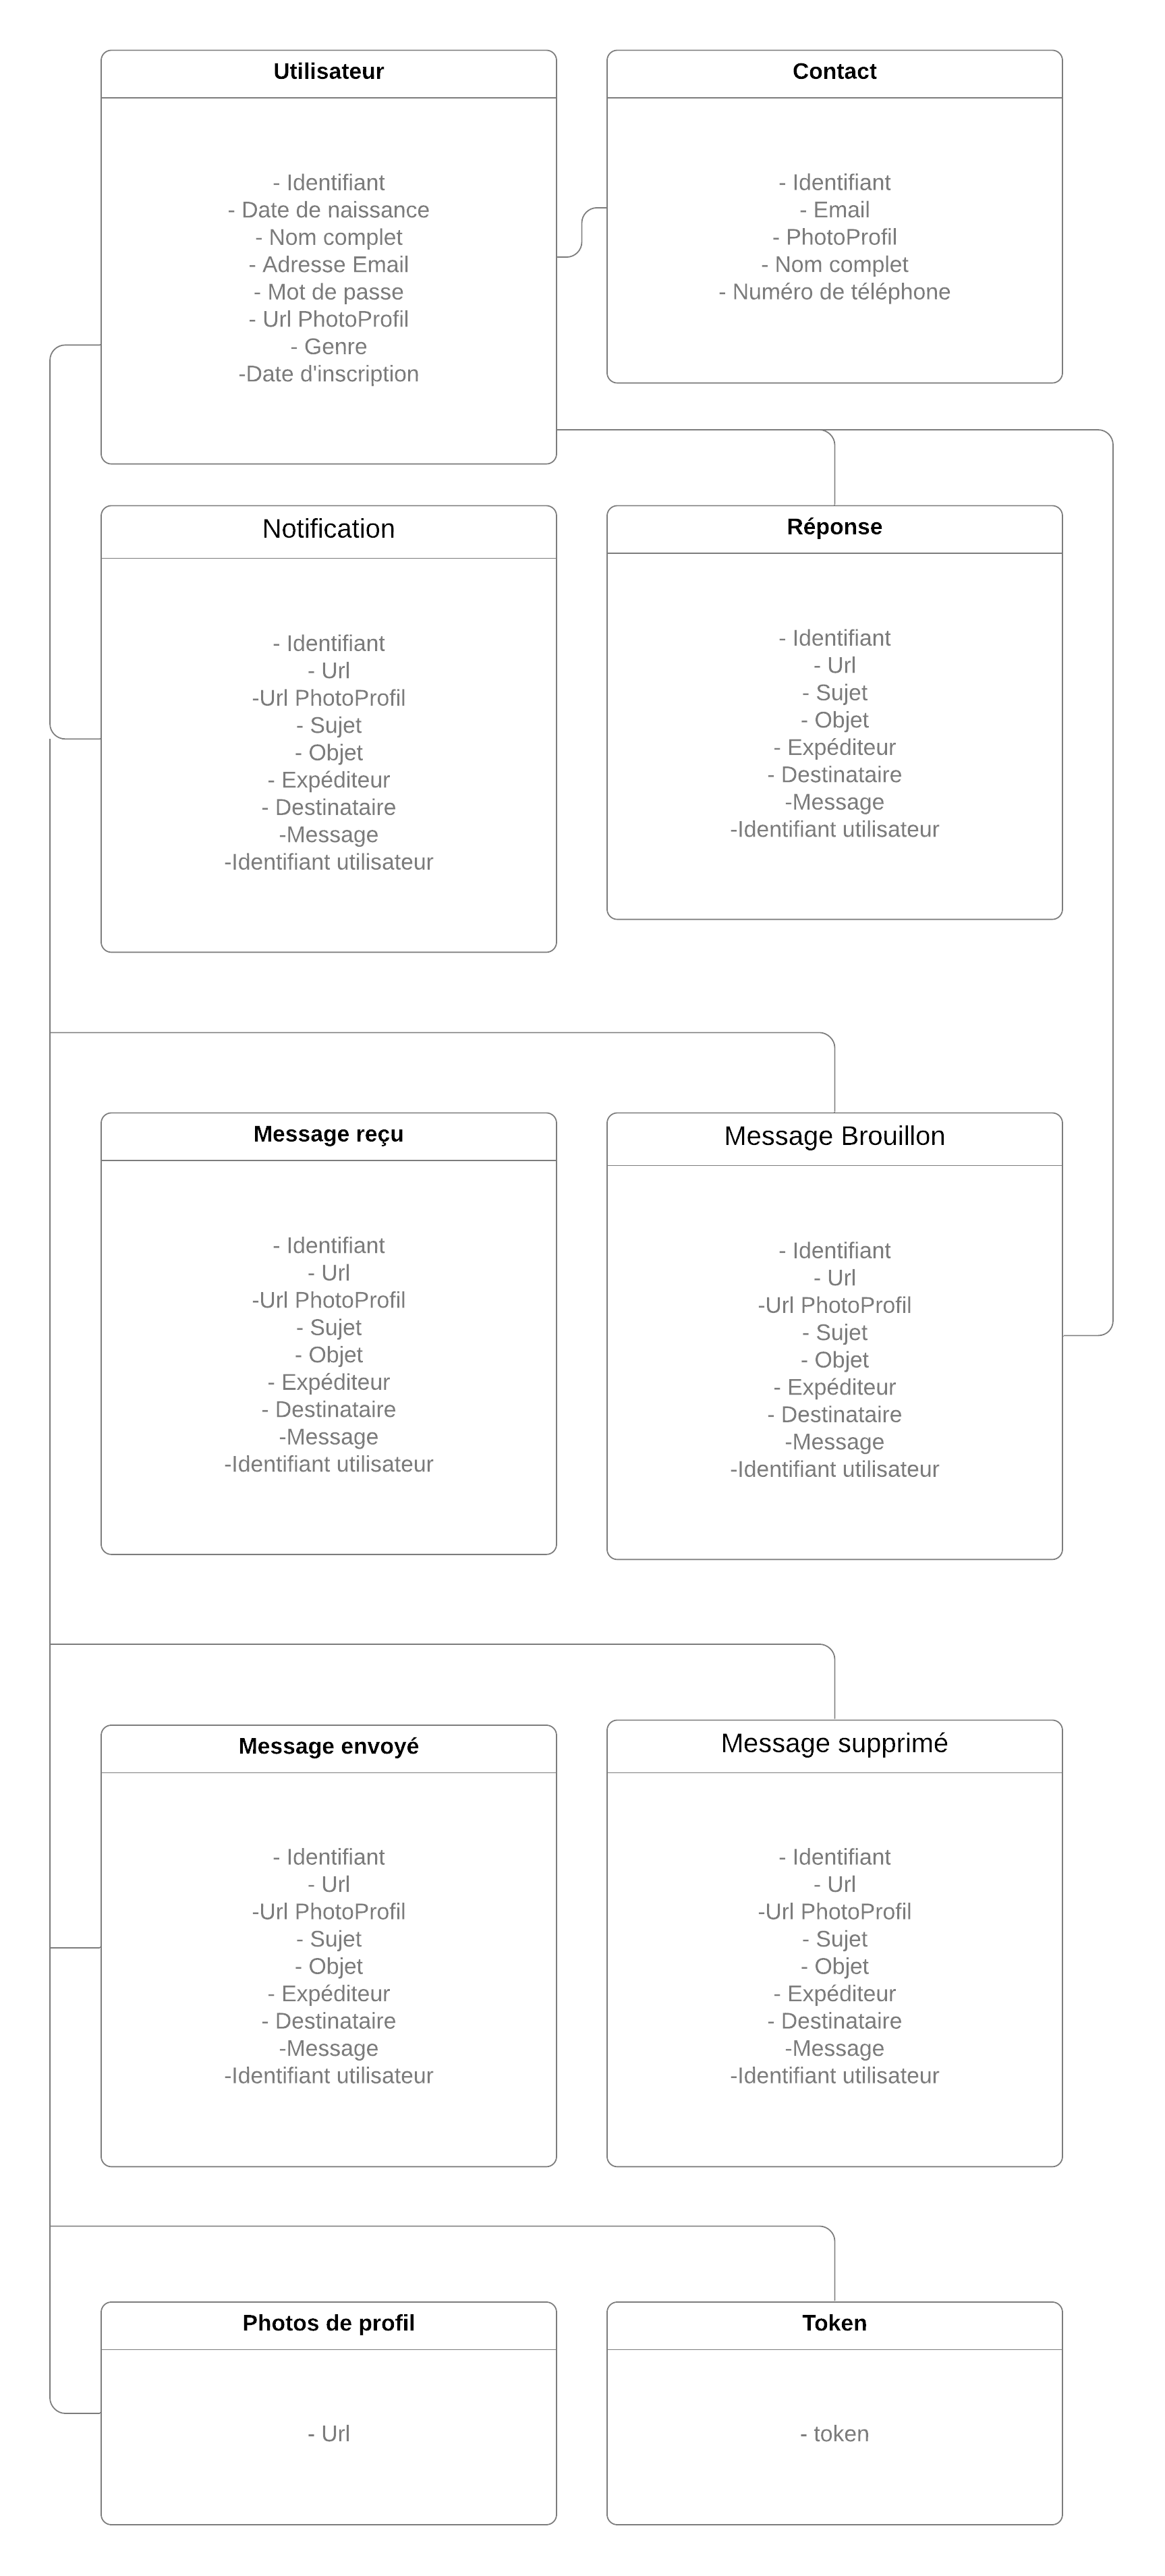
\includegraphics[scale=0.18 ]{Représentation simplifiée de notre base de données}
    \caption{Représentation simplifiée de notre base de données}
    \label{fig:Representation}
\end{figure}
\section{\huge La Modélisation de notre application :}
\subsection{\LARGE Diagramme des cas d'utilisation }
\LARGE L'objectif de ce diagramme de cas d'utilisation est de montrer globalement comment l'utilisateur pourra interagir avec notre projet une fois finalisé.\\
\begin{figure}[H]
    \centering
    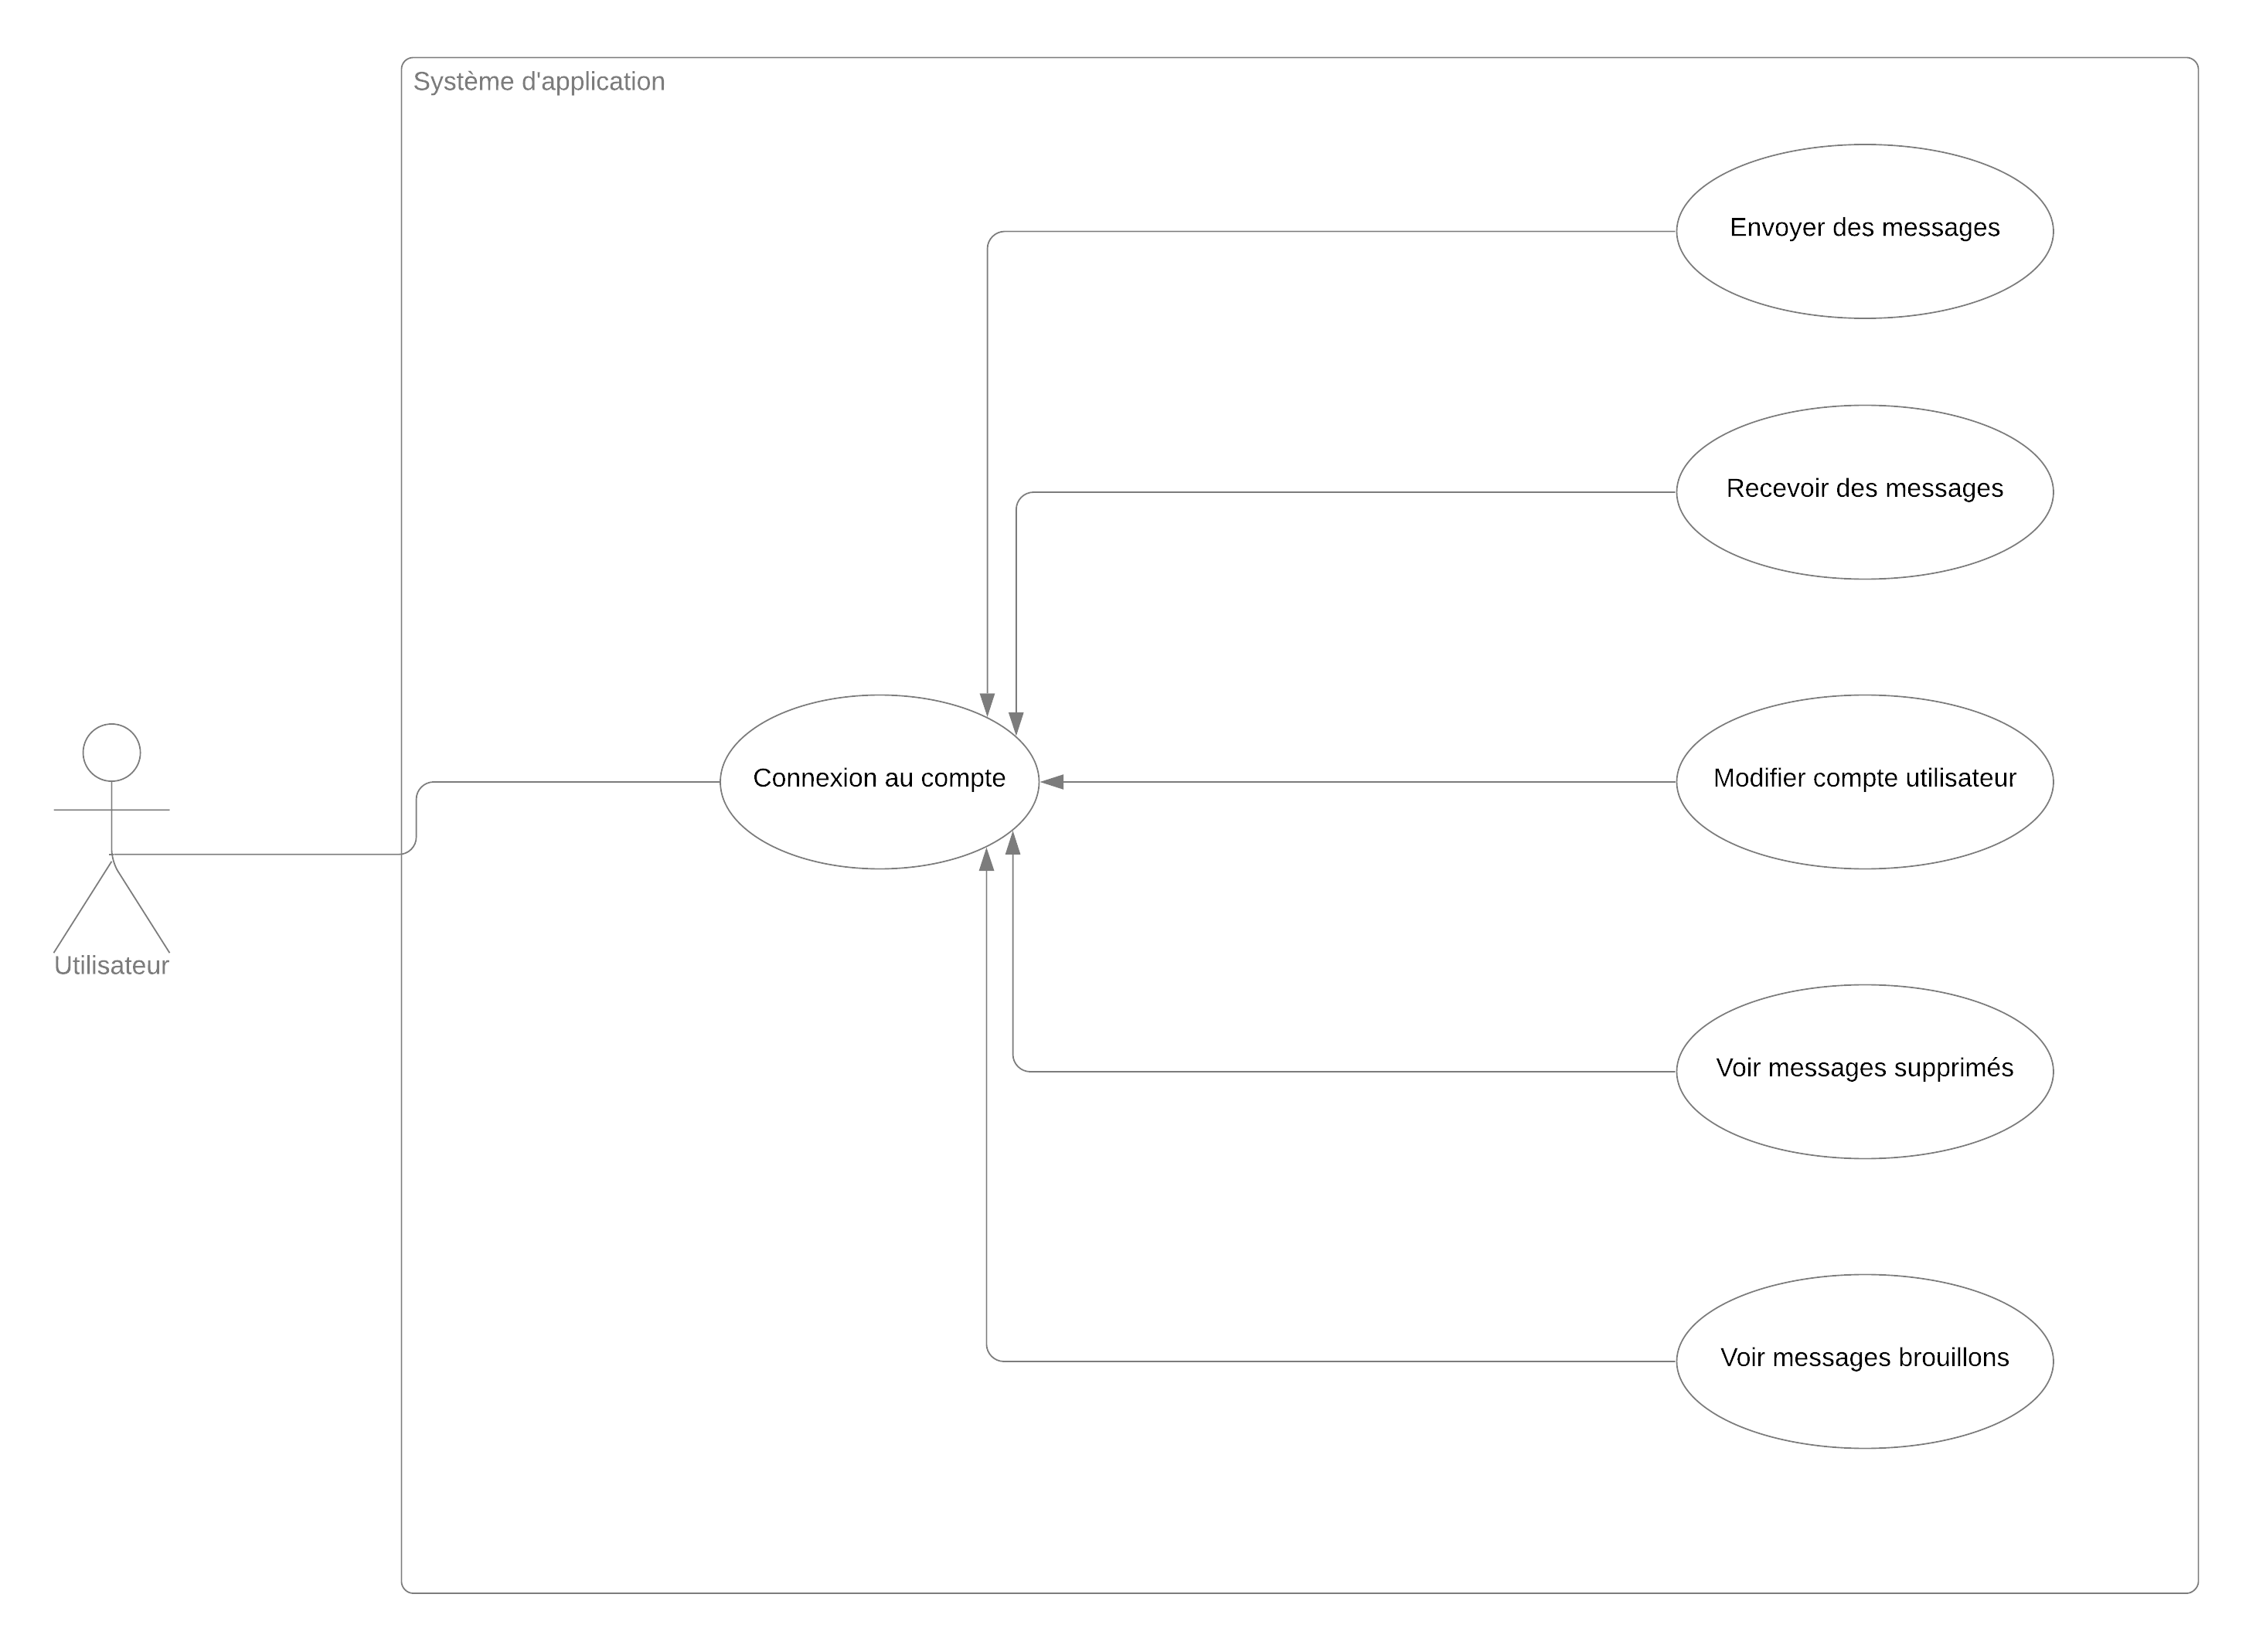
\includegraphics[width=1\textwidth]{DCU}
    \caption{Diagramme des cas d'utilisation}
    \label{fig:DCU}
\end{figure}
\subsection{\LARGE Diagramme d'activité (UML)}
\LARGE Dans UML, un diagramme d’activité est utilisé pour afficher la séquence des activités. Les diagrammes d’activité représentent le flux de travail à partir d’un point de départ au point d’arrivée. Détaillant les nombreux sentiers de décision, qui existent dans la progression des événements contenus dans l’activité. Ils peuvent être utilisés à des situations de détail, où le traitement parallèle peut survenir dans l’exécution de certaines activités.\\\\
Ce diagramme ci-dessous est le diagramme d'activité de notre activité principale (authentification), cette activité est présentée à l'utilisateur lors de la première ouverture de l'application, l'utilisateur peut alors interagir avec cette activité en se connectant ou en créant un compte.\\\\
Le déplacement entre ces activités est déterminé automatiquement par l'application en fonction des actions précédentes de l'utilisateur.
\begin{figure}[H]
    \centering
    \includegraphics[width=1\textwidth]{Diagramme d'activités}
    \caption{Diagramme d'activités principales}
    \label{fig:activity}
\end{figure}
Après l'accès au compte, l'utilisateur pourra interagir avec l'application et toutes les données en relation avec son compte en utilisant d'autres activités.
\subsection{\LARGE Conclusion}
\LARGE Cette partie nous a permis d'acquérir les connaissances nécessaires sur les différents défis auxquels nous sommes confrontés dans notre projet et a façonné notre vision de notre application et nous a aidés à identifier ses besoins.\\
Dans le chapitre suivant, nous passerons à l'implémentation de notre application en utilisant le langage de programmation choisi (JAVA) et l'IDE Android Studio.
\printindex
\newpage
\end{titlepage}
\end{document}